\documentclass[main.tex]{subfiles} % Subfile-Class


% ============================================================================== %
%                            Subfile document                                    %
% ============================================================================== %

\begin{document}

% Template

\subsubsection{Antriebe und Dimensionierung}

Dieser Abschnitt beschäftigt sich mit der Auswahl eines passenden Antriebs
mitsamt Steuerung für den Pfadfinder. Die Evaluation der Antriebe, siehe
Anhang~\ref{appendix:Antriebe}, hat ergeben, dass ein Schrittmotor der Firma
DFRobot, siehe Abbildung~\ref{Schrittmotor_FIT0278}, eingesetzt wird. Dieser
ist in der Lage, mit 1.7A den Pfadfinder auf bis zu $2\frac{m}{s}$ zu
beschleunigen.

\begin{figure}[H]
    \centering
    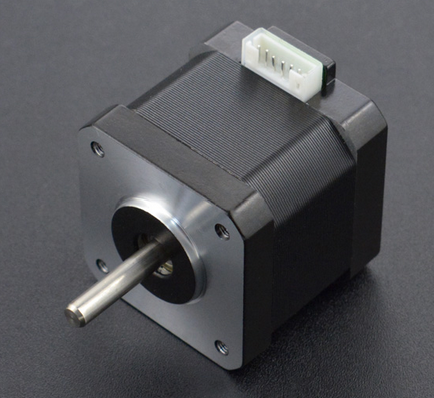
\includegraphics[width = 0.25 \linewidth]{fig_Antriebe_und_Dimensionierung/DFRobot_Stepper_FIT0278.png}
    \caption{Schrittmotor}~\label{Schrittmotor_FIT0278}
\end{figure}

\begin{figure}[H]
    \centering
    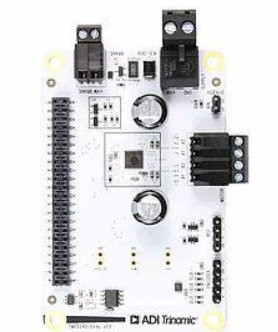
\includegraphics[width = 0.25 \linewidth]{fig_Antriebe_und_Dimensionierung/TMC_5240_EVAL.png}
    \caption{Evaluationboard TMC5240}~\label{Schrittmotorentreiber_EVAL}
\end{figure}

Angesteuert werden diese Motoren über einen Vollintegrierten
Schrittmotorentreiber der Firma ADI-Trinamic. Um weniger Entwicklungsaufwand zu
haben, wird auf 2 Evaluation-Boards des Treiber-IC's \textit{TMC-5240}
zurückgegriffen, gezeigt in Abbildung~\ref{Schrittmotorentreiber_EVAL}. Eines
der Team-Mitglieder hat bereits Erfahrungen mit diesem speziellen Treiber und
kann auf entsprechende Treiber-Evaluation-Boards aus seinem beruflichen Umfeld
zurückgreifen.

Die Abbildung~\ref{Ansteuerungstopologie_Schrittmotorentreiber} zeigt
schematisch, wie diese Treiber angesteuert werden.

\begin{figure}[H]
    \centering
    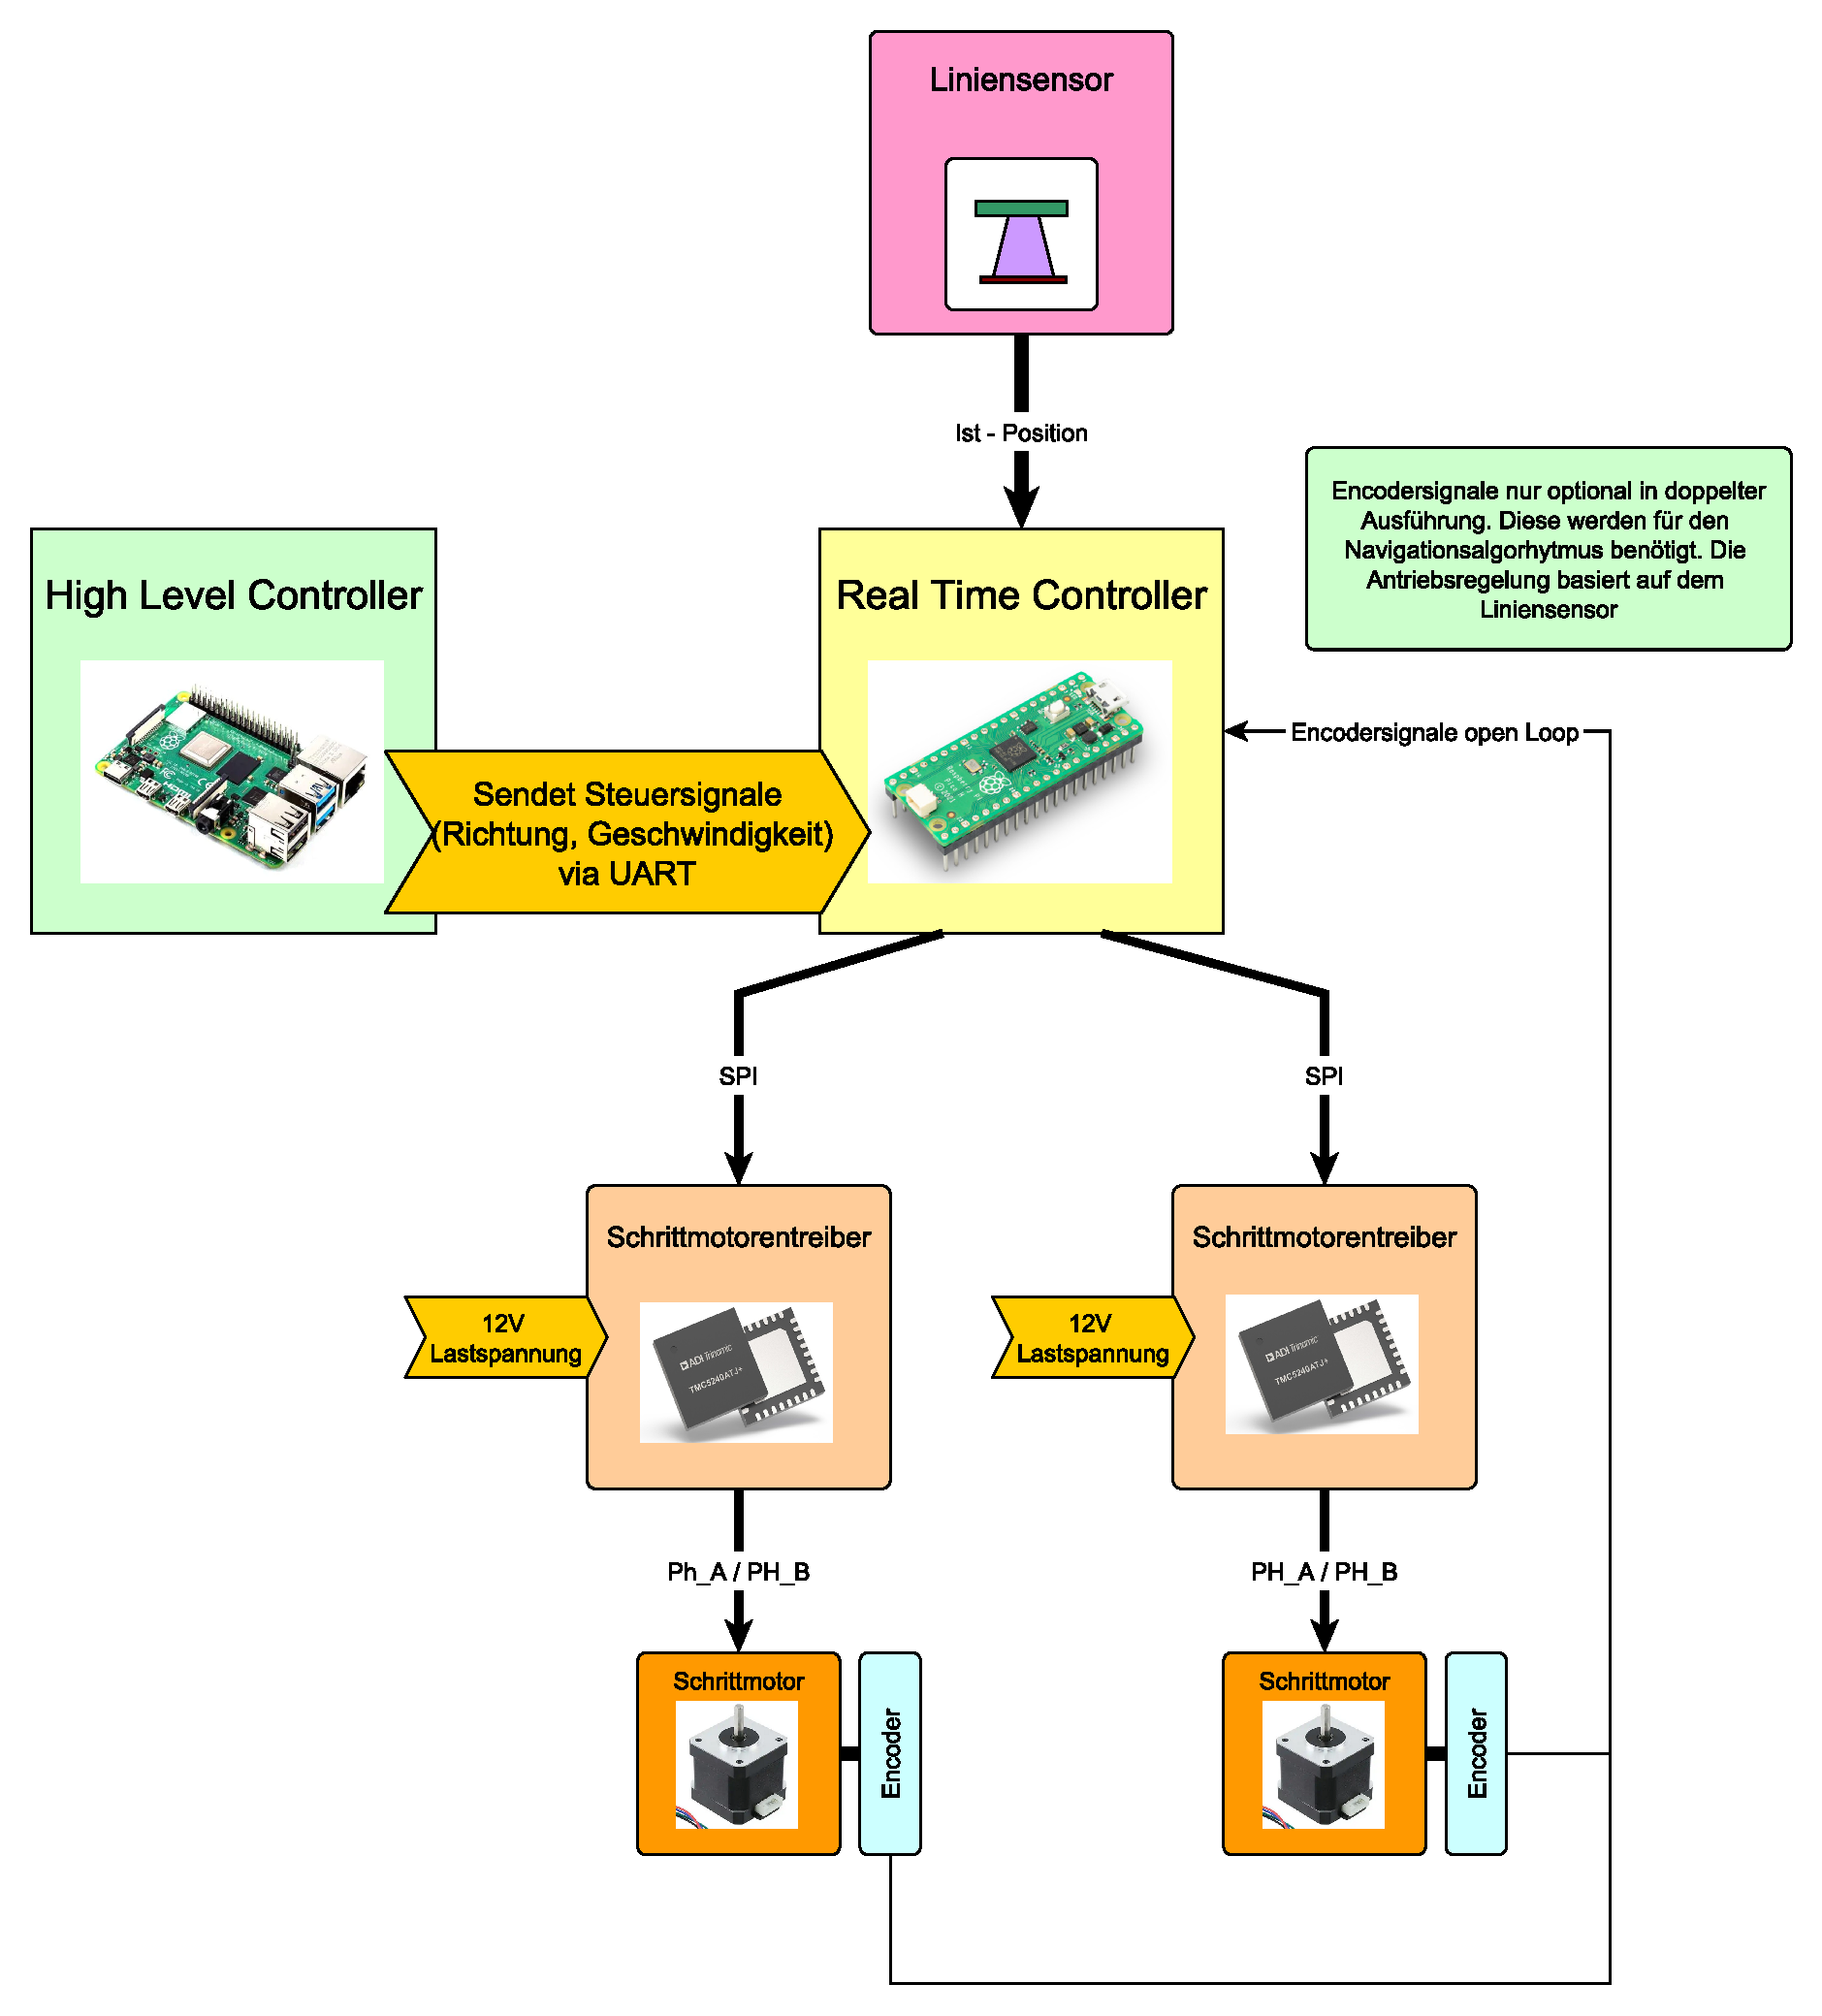
\includegraphics[width = 1\linewidth]{fig_Antriebe_und_Dimensionierung/Konzept_RTC_Trinamic.pdf}
    \caption{Ansteuerungstopologie Schrittmotoren}~\label{Ansteuerungstopologie_Schrittmotorentreiber}
\end{figure}

Die Antriebsregelung wird im Sinne der Gewaltenteilung auf einem eigenen PCB
umgesetzt. Eingangssignale für diesen sind der Liniensensor und 1 oder sogar 2
Encoder. Die Regelung findet allerdings ohne Encoder statt. Die Einganggrösse
dafür ist lediglich die Position des Fahrzeugs auf der Linie. Angesteuert
werden die Schrittmotorentreiber über den SPI-Bus des Mikrocontrollers.

Die Encoder werden benötigt, damit der Navigationscomputer nachvollziehen kann,
welche Strecke zurückgelegt wurde. Aus Gründen der Echtzeitfähigkeit beim
Auszählen der Encoder werden diese allerdings trotzdem auf der
Antriebssteuerung ausgewertet. Die Encoder sind zum aktuellen Stand des
Projekts eine Fallback-Lösung. Im Nachfolgemodul wird noch evaluiert, ob die
getätigten Schritte, welche aus dem Motorentreiber ausgelesen werden können,
ausreichen können, um die gefahrene Strecke nachvollziehen zu können.

Signale, in welche Richtung das Fahrzeug bewegt werden soll, sowie Start- und
Stopp-Signale erhält der Mikrocontroller vom Navigationscomputer über eine
UART-Schnittstelle. Der Greifer-Controller kann dem Antriebs-Controller
ebenfalls via UART, Signale übermitteln, welche die Antriebe anhalten - das
Fahrzeug drehen oder eben weiterfahren lassen.

Abbildung~\ref{fig:Blockschaltbild_Motioncontroller}zeigt schematisch, welche
Funktionsgruppen das entsprechende PCB enthält.

\begin{figure}[H]
    \centering
    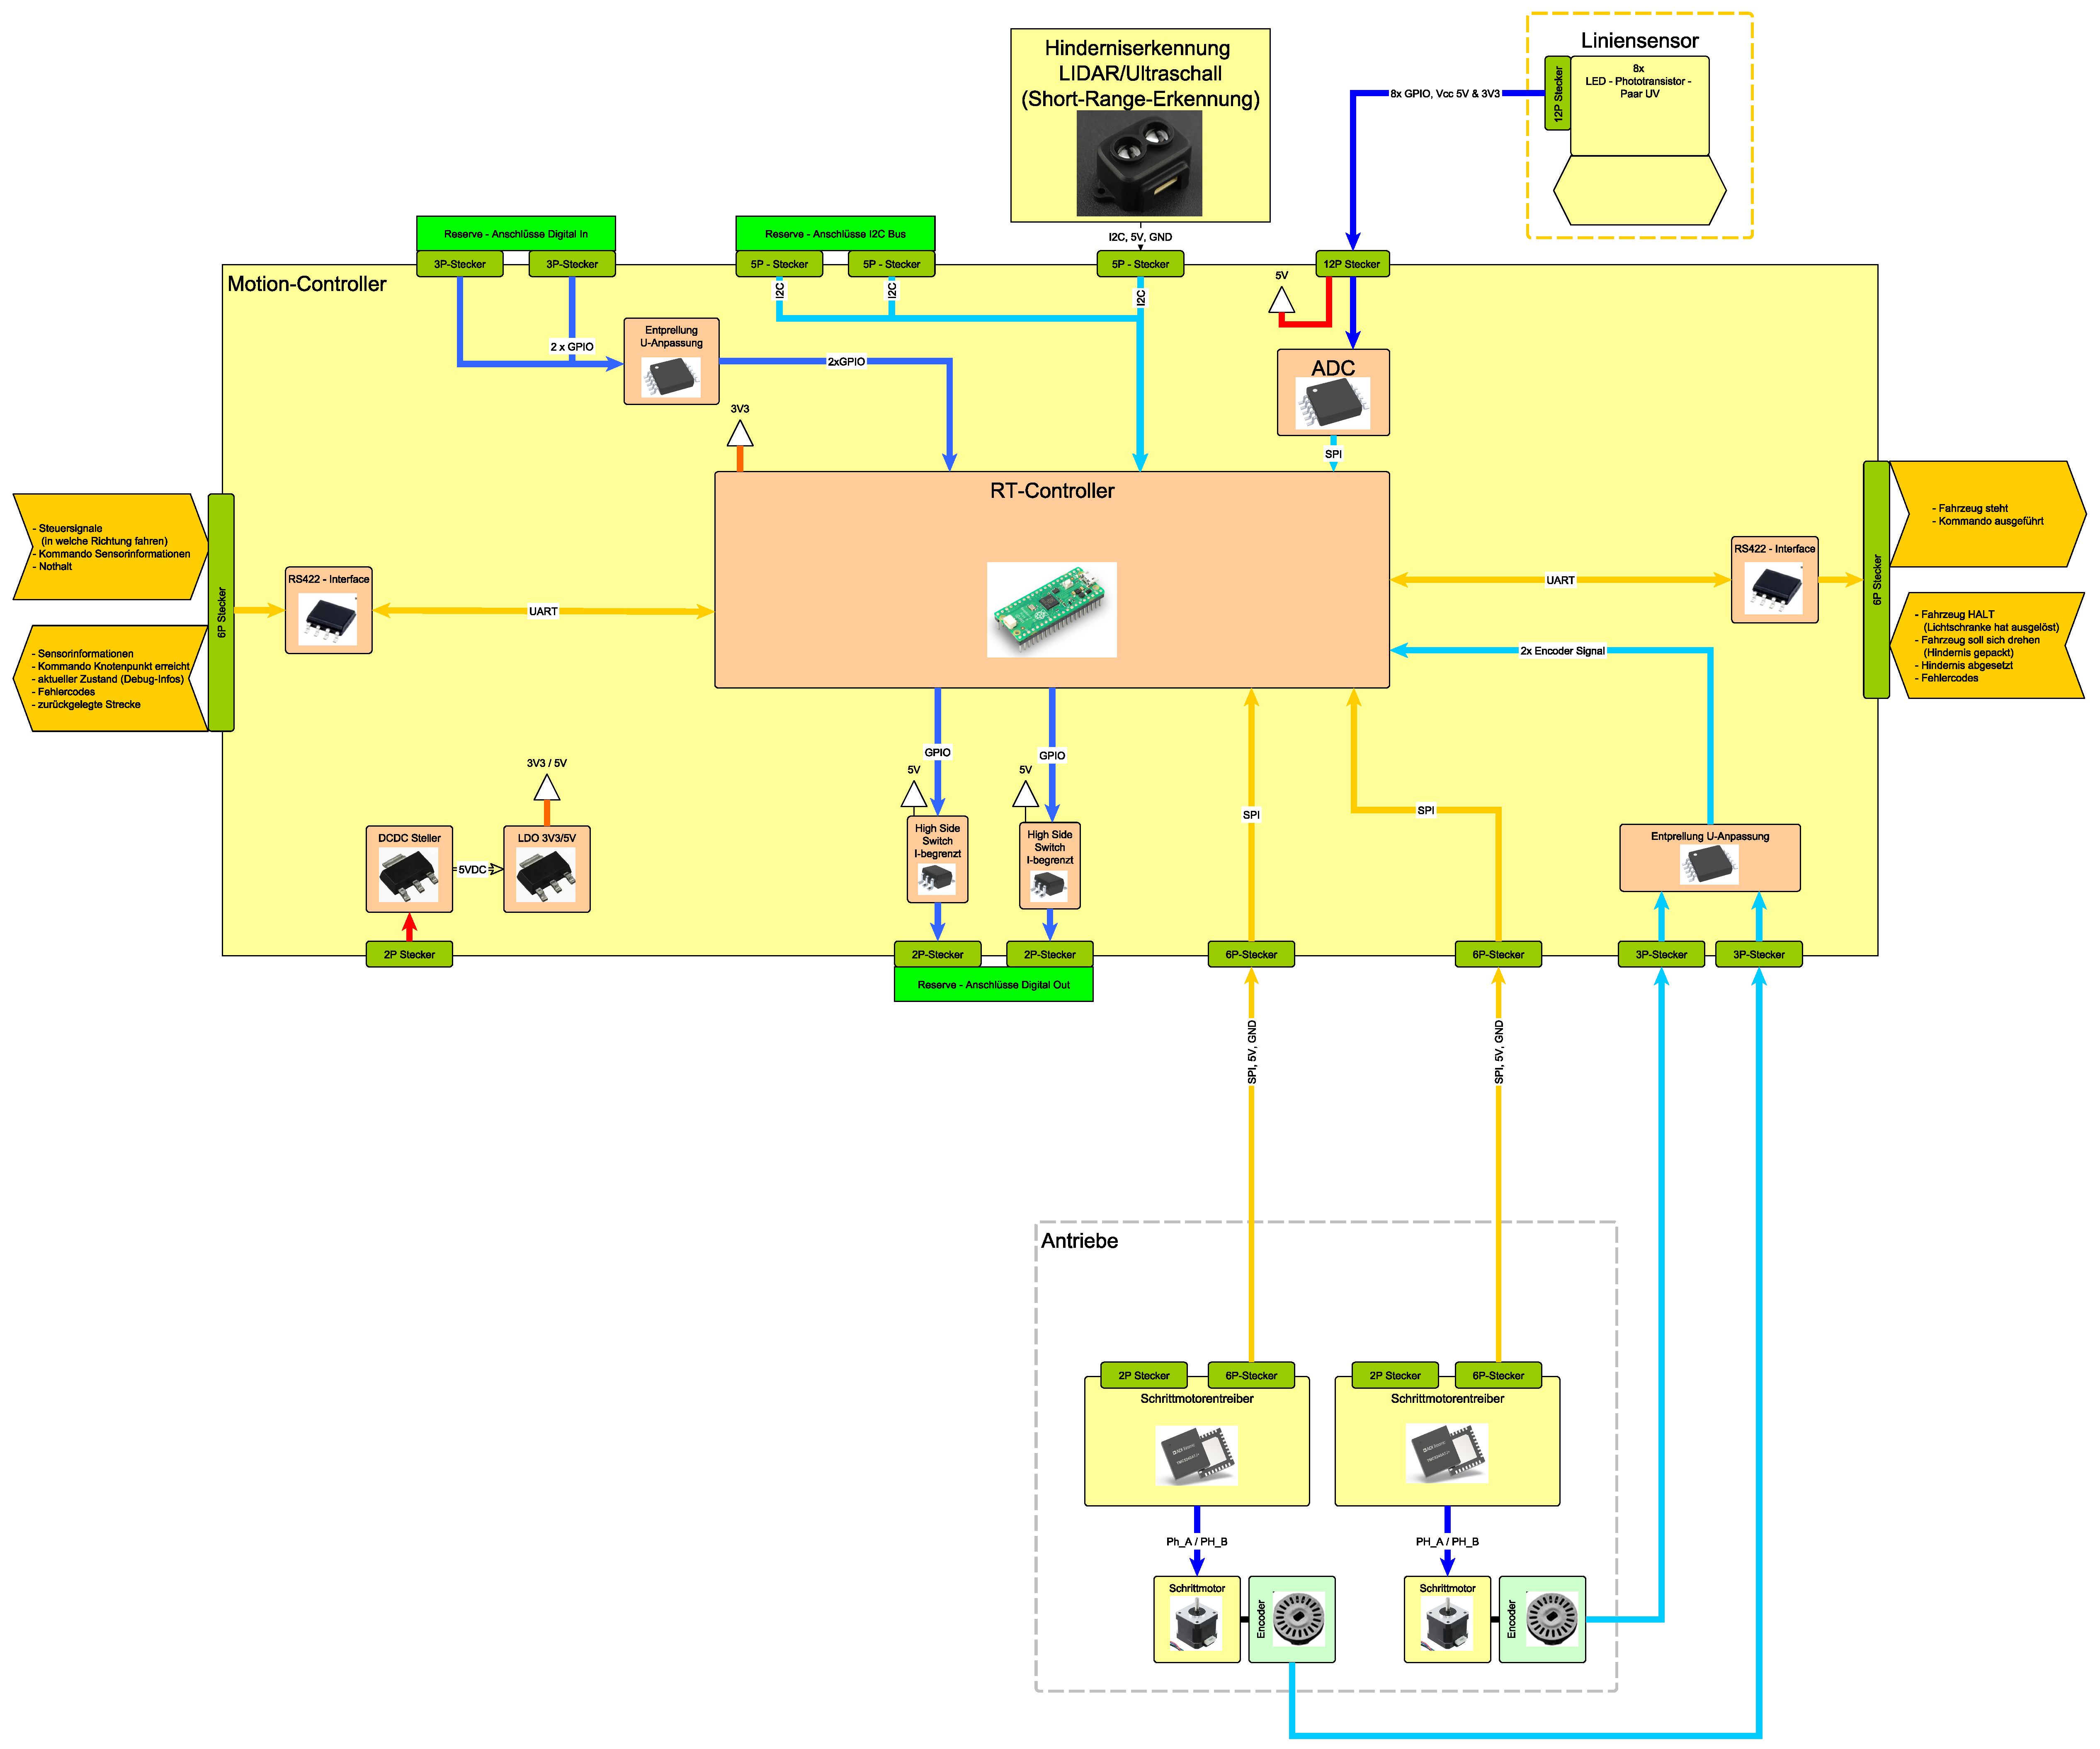
\includegraphics[width = 1\linewidth]{fig_Antriebe_und_Dimensionierung/MotionController_Blockschaltbild.pdf}
    \caption{Blockschaltbild Motion Controller}~\label{fig:Blockschaltbild_Motioncontroller}
\end{figure}

Der Motion Controller besitzt sowohl digitale Eingänge als auch Ausgänge mit
umschaltbaren Spannungsniveaus als Reserve, falls im Laufe des Folgemoduls
PREN2 Sensorik angepasst oder zusätzliche Aktorik hinzugefügt werden muss.

Abbildung~\ref{fig:MotionBoard_PCB} zeigt das Motion-Controller-PCB in einer
3D-Ansicht. Es besitzt 3 I2C - Verbindungen, ein spezielles HC-SR04
Ultraschallsensor Interface sowie die erwähnten digitalen Ein-/Ausgänge.
Darüber hinaus ist eine Schnittstelle für den Liniensensor vorgesehen und
ausserdem ein Gyroskop zur Winkelerfassung verbaut. Es wird wie eine Brücke auf
die beiden Evaluation-Boards von Trinamic aufgesteckt sein, wofür sich an den
äusseren Rändern die breiten Steckerleisten befinden.

\begin{figure}[H]
    \centering
    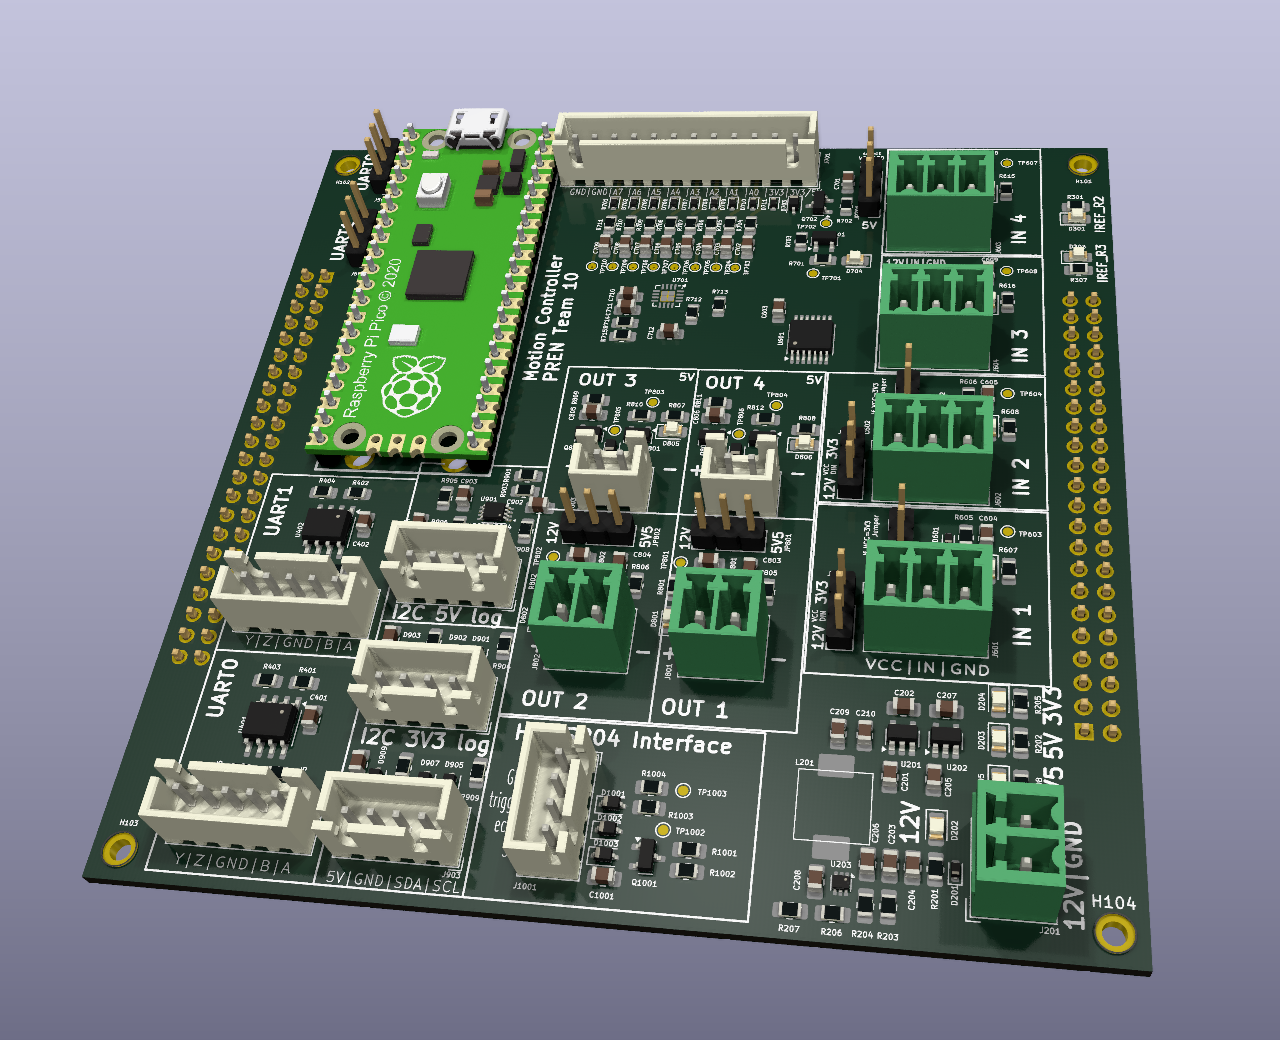
\includegraphics[width = 0.75\linewidth]{fig_Antriebe_und_Dimensionierung/MotionControllerPCB.jpg}
    \caption{3D-Ansicht Motion Controller}~\label{fig:MotionBoard_PCB}
\end{figure}

\end{document}

Stand des Konzeptes zu PREN1 wäre dieser Controller in der Lage, die Aufgabe
des Greifers ebenfalls zu übernehmen. Da allerdings nicht klar ist, wie gut der
Greifer zu seinem aktuellen Stand umgesetzt werden kann und ob es noch mehr
Ein-/Ausgänge benötigt. Daher wird fürs erste ein eigenes PCB für diese Aufgabe
vorgesehen.